%!TEX root = main.tex
\section{Introduction}% 

\par 
With the ever-increasing complexity 
and size of datasets,
there is a growing demand for 
information visualization tools
that can help data scientists make sense of large
volumes of data.
Visualizations help discover 
trends and patterns, 
spot outliers and anomalies, 
and generate or verify hypotheses.
Moreover, 
visualizations are accessible and intuitive: 
they tell us stories about our data; 
they educate, delight, inform, 
enthrall, amaze, and clarify.
This has led to the overwhelming popularity
of point-and-click visualization tools like Tableau~\cite{Stolte2002},
as well as programmatic toolkits like ggplot, D3, Vega, and matplotlib. 
We term these tools as {\em visualization-at-a-time} approaches, since
data scientists need to individually 
generate each visualization (via code or interactions),
and examine them, 
one at a time.


\par
As datasets grow in size and complexity, 
these visualization-at-a-time approaches start to break down,
due to the limited time availability on the 
part of the data scientists---there 
are often too many visualizations to examine for a given 
task, such as identifying outliers, or inferring patterns. 
Even on a single table, 
visualizations can be generated
by varying the subsets of data operated on, 
or the attributes (or combinations
thereof) that can be visualized. 
If we add in various visualization modalities, encodings,
aesthetics, binning methods, and transformations,
this space becomes even larger. 
(For this work, we focus primarily on
the impact of varying the data subsets
and attributes visualized---some of these
latter concerns are the focus of recent work~\cite{Wongsuphasawat2017}.)

\begin{wrapfigure}{l}{0.4\textwidth}
\centering
\vspace{-10pt}
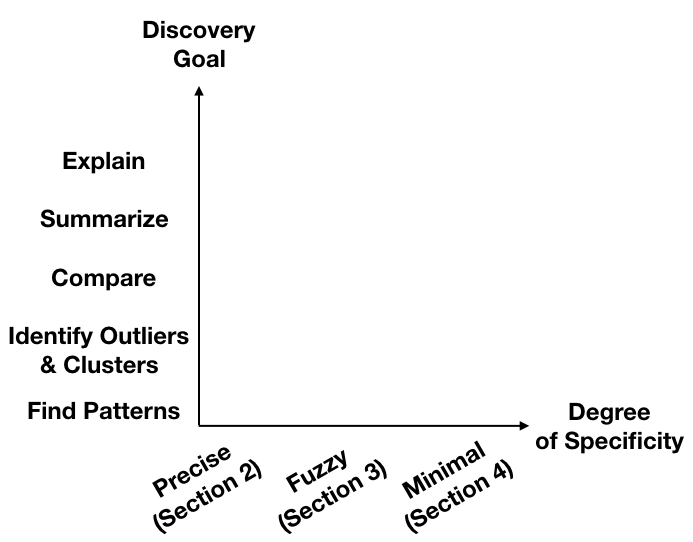
\includegraphics[width=\linewidth]{figures/dimensions_cropped.png}
\vspace{-15pt}
\caption{The two dimensions of discovery settings. The Y axis depicts the different discovery goals ordered in roughly increasing complexity, while the X axis characterizes decreasing levels of query specificity and correspondingly increasing levels of autonomous assistance.}\label{fig:dimensions}
\vspace{-15pt}
\end{wrapfigure}


\par
Thus, there is a pressing need for an 
intelligent,
interactive, understandable, usable, and
enjoyable tool that can help 
data scientists navigate
collections of visualizations, across a range of possible analysis goals and modalities that data scientists may require.
We term our hypothesized comprehensive tool \vida,
short for {\em VIsual Discovery Assistant}.
Data scientists can specify any discovery
goal at a high level, in one of many intuitive input modalities supported in \vida, with \vida automatically traversing visualizations to provide solution or guidance for the
specified discovery goal, thereby
eliminating the tedium and wasted
labor of comparable visualization-at-a-time 
approaches.

\par
\stitle{\vida Dimensions.} 
In order to be a holistic solution for 
navigating collections of visualizations,
\vida must be able to support various discovery
settings. 
We organize these settings along two
dimensions, displayed along the Y axis and 
X axis (respectively) of Figure~\ref{fig:dimensions}---first, 
the overall discovery goal,
and second, the degree of specificity of the goal.



\par
 We identify five 
common discovery goals in visual data exploration, organized
along the Y axis:
{\em finding patterns}, {\em identifying anomalies/clusters}, {\em summarizing}, 
{\em performing comparisons}, {\em providing explanations}.
These five goals borrow from functionalities in existing
systems, as well as related visualization task taxonomies~\cite{Amar2005,Heer2012}.
They are organized along the Y axis in a sequence of roughly increasing complexity; however, we must emphasize that these goals are distinct from one other. 
We omit low-level goals such as filtering or sorting, since these functionalities are common in existing visualization-at-a-time tools and toolkits. We also omit goals that go beyond visual data exploration, such as extrapolation, supervised learning, and cleaning, among others. 

\begin{wrapfigure}{r}{0.5\textwidth}
\centering
\vspace{-15pt}
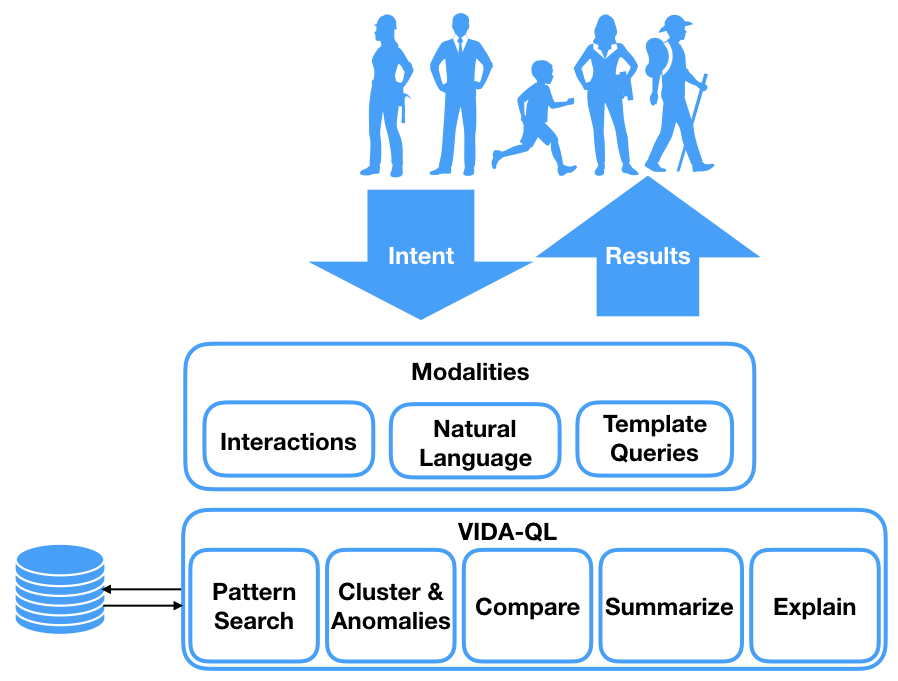
\includegraphics[width=\linewidth]{figures/VIDA_architecture.png}
\vspace{-25pt}
\caption{\vida Architecture\label{fig:vida_architecture}
\vspace{-15pt}
}
\end{wrapfigure}


\par 
 We identify three degrees of specificity
for the query input, organized along the X axis:
{\em precise}, {\em fuzzy}, {\em minimal}.
The degree of specificity characterizes the division
of work between how much user has to specify
versus how much the system has to automatically
infer and aid in accomplishing the discovery goal. 
For the precise setting, the onus is placed on the user
to provide an exact and complete specification of 
what the solution to their discovery
goal must look like;
for the fuzzy setting, the user can provide
a vague specification of what the solution must look like;
and finally, for the minimal setting,
the user provides a minimal specification, or
leaves the characteristics of the solution underspecified,
leaving it up to the system to ``fill in'' the rest.
As we proceed along the X axis,
it gets harder for the system to automatically
interpret what the user might have in mind as a solution
to their goal.


% \begin{table}[!t]
% \scriptsize
% \centering
% \begin{tabular}{l|l|l|l|l|l}
% & \multicolumn{5}{c}{Discovery Goals}                                                                     \\ \hline
% & Find Patterns & Identify Anomalies and Clusters      & Compare           & Summarize  & Explain          \\ \hline
% Precise (Section~\ref{sec:precise}) & \multicolumn{3}{c|}{Zenvisage~\cite{Lee2017}, ZQL~\cite{Siddiqui2016}}                                      &            &                  \\ \hline
% Fuzzy (Section~\ref{sec:vague})     & ShapeSearch\cite{Siddiqui2018}   & Scorpion\cite{Wu2013}, Profiler~\cite{Kandel2012}, Natural Language & Natural Language~\cite{Fast2018,Setlur2016,Hoque2017}  &            & Natural Language \\ \hline
% Minimal (Section~\ref{sec:minimal}) &               & \multicolumn{1}{c|}{Storyboard~\cite{Lee2018}}      & SeeDB~\cite{Vartak2015}, Storyboard & Storyboard & Storyboard      
% \end{tabular}
% \caption{Overview of the systems described in this paper. Columns are organized into discovery goals and rows are ordered by decreasing levels of query specificity and correspondingly increasing levels of autonomous assistance.\agp{fix this. add specificity, augment references}}\label{fig:table}
% \end{table}



% & \multicolumn{5}{c}{Discovery Goals}                                                                     \\ \hline
% & Find Patterns & Identify Anomalies and Clusters      & Compare           & Summarize  & Explain          \\ \hline
% Precise (Section~\ref{sec:precise}) & \multicolumn{3}{c|}{Zenvisage~\cite{Lee2017}, ZQL~\cite{Siddiqui2016}}                                      &            &                  \\ \hline
% Fuzzy (Section~\ref{sec:vague})     & ShapeSearch\cite{Siddiqui2018}   & Scorpion\cite{Wu2013}, Profiler~\cite{Kandel2012}, Natural Language & Natural Language~\cite{Fast2018,Setlur2016,Hoque2017}  &            & Natural Language \\ \hline
% Minimal (Section~\ref{sec:minimal}) &               & \multicolumn{1}{c|}{Storyboard~\cite{Lee2018}}      & SeeDB~\cite{Vartak2015}, Storyboard & Storyboard & Storyboard      
% \end{tabular}
% \caption{Overview of the systems described in this paper. Columns are organized into discovery goals and rows are ordered by decreasing levels of query specificity and correspondingly increasing levels of autonomous assistance.\agp{fix this. add specificity, augment references}}\label{fig:table}
% \end{table}



\par
\stitle{\vida Input Modalities.} To support the spectrum of 
demands imposed by the
discovery settings described above, \vida 
must support a range of interactive input modalities,
as displayed in Figure~\ref{fig:vida_architecture},
catering to a range of user expertise and preferences.
These input modalities include: 
\squishlist
	\item interactions, either with an existing visualization, such as brushing-and-linking or hovering, or those that construct a new one, such as drag-and-drop or sketching; and
	\item restricted template queries, involving selection of operators and operands from a drop-down menu; and
	\item natural language, via a keyword search box, dialog, or conversational interface.
\squishend
Each of these inputs are compiled down
into a query in a query language, called \vidaql.
Alternatively, expert users may directly invoke \vidaql queries.
\vidaql queries will natively support the five discovery goals and combinations thereof, e.g., summarization followed by pattern search. Another important element is how much does a user actively requests for visualizations (``pull'') versus how much \vida recommends visualizations (``push''). Given that we expect \vida to support a range of specificities, \vida must support both push and pull, with pull decreasing in importance and push gaining importance, as we go from the precise to minimal setting.



% Common framework and module means there are underlying functionalities can be shared (e.g. statistical modules, data heavy-lifting operations)
% - From the top: many different types of users (novices/experts), each with some high-level intent in one of the following modalities:
%      - Interaction: produces as an output either through the creation a visualization (e.g. sketching, drag-and-drop) or changes upon a visualization (e.g. brushing, selections, clicks)
%      - Partial specification includes some minimal input such as input X,Y of interest
%      - Either that or user can directly specify their query exactly in VIDA-QL
% - VIDA-QL contains 5 discovery modules which each have their own "push and pull" components, i.e. work with both search and recommend.


\par
\stitle{Present Day Visual Query Systems.}
We have described \vida so far as if no comparable capabilities
exist today.
This is not the case; in Table~\ref{fig:table}, we list some examples of systems
that partially provide the functionality of \vida,
for certain settings and input modalities.
We will describe some of these systems later on in the paper. 
Since all of these systems allow users to query data {\em visually},
we call these systems {\em Visual Querying Systems}, or VQSs for short.
VQSs typically {\em (i)} 
employ objectives that are perceptually-aware,
taking into account for the fact that the results are typically
consumed by a human analyst, rather than an algorithm;
{\em (ii)} provide some interactive interface or declarative capabilities
to express the discovery goal as a ``what'' rather than a ``how'';
and {\em (iii)} possess optimization capabilities to facilitate
the efficient discovery of visual insights. 


\begin{table}[!t]
\scriptsize
\centering
\begin{tabular}{l|l|l|p{7.5cm}}
VQS & Discovery Goals Covered & Specificity & Interactions Supported \\ \hline

Zenvisage~\cite{Lee2017,Siddiqui2016} & Find Patterns, Cluster/Outliers, Compare & Precise & Interactions (Clicking, Sketch, Drag-and-drop), Query Language \\
TimeSearcher~\cite{hochheiser2004dynamic} & Find Patterns, Cluster/Outliers & Precise & Interactions (Clicking, Sketch) \\ 
Query-by-Sketch~\cite{wattenberg2001sketching} & Find Patterns & Precise & Interactions (Clicking, Sketch) \\ 

Scorpion~\cite{Wu2013} & Explain & Fuzzy & Interactions (Clicking) \\

ShapeSearch~\cite{Siddiqui2018} & Find Patterns & Fuzzy & Interactions (Sketch), Natural Language, Query Language \\

%Data Polygamy~\cite{chirigati2016data} & Compare, Explain & Fuzzy & Query Language \\
Profiler~\cite{Kandel2012} & Compare & Fuzzy & Interactions (Clicking, Brushing-and-Linking) \\
SeeDB~\cite{Vartak2015} & Compare & Minimal & Interactions (Clicking) \\
Storyboard~\cite{Lee2018} & Cluster/Outliers, Compare, Summarize & Minimal & Interactions (Clicking) \\
iDiff~\cite{Sarawagi1998,Sarawagi2000} & Compare, Explain & Minimal & Query Language \\

\end{tabular}
\vspace{-10pt}
\caption{A Sample of Visual Query Systems}\label{fig:table}
\vspace{-10pt}
\end{table}


\par
\stitle{Outline.}
The rest of our paper is organized along the degree of specificity
of discovery goal, and we will allude to the specific discovery
goals as well as input modalities as we go along. 
The degree of input specificity is the factor
that most significantly affects the architecture of \vida,
with the complexity increasing as the specificity decreases---in that
the system has to do more ``guesswork'' to support underspecified goals. 


\par We begin by discussing the 
the {\em precise} setting (Section~\ref{sec:precise}).
We describe \zv~\cite{Siddiqui2016} 
as a partial solution for
this setting, and thereby a starting point for \vida,
partially eliminating the problem
of having to manually examine large numbers 
of visualizations for a given discovery goal, 
which can be error-prone and inefficient.

\par However, a design study using \zv demonstrates
that the precise setting is insufficient for
addressing all of the demands of real-world use-cases~\cite{Lee2017}.
In particular, users do not have
a clear understanding of their querying intent without looking at example visualizations or summaries of the data, and even when they do, their intent involves
vague or high-level notions that can not be expressed clearly.

\par To bridge the gap between the user's high-level
intent and the system demands,
we outline a set of research challenges
that goes beyond simple precise visual querying, by
(a) supporting a wider class of vague or ``fuzzy'' high-level
queries, thereby increasing the expressiveness
of \vida (Section~\ref{sec:vague});
and 
(b) making it easier to know what to query
by recommending visualizations that provide
a high-level understanding of the data (Section~\ref{sec:minimal}).

\stitle{Interfaces and Interactions, not Optimization.}
In this paper, we focus our attention on the interfaces,
query languages, and capabilities, 
and how to use them to capture discovery goals
with varying degrees of specification, as opposed to optimization.
Indeed, once the query is issued in some form 
(say, translated into a \vidaql
query),
optimization is crucial to try to traverse the space 
of visualizations and return results in an interactive manner.
A range of techniques may be adopted for this purpose,
including parallelism, multi-query optimization, sampling,
pruning, and pre-computation~\cite{Siddiqui2016,Vartak2015}.
We expect a similar combination of techniques to be applicable to
each of the settings that we consider. To limit the scope of this paper, we have
decided to avoid describing optimization aspects and focus on the interfaces and interactions instead.


% \dor{Our discussion in this paper focuses on the interface and interactions, rather than optimizations (sampling, pruning, etc.) commonly used in VQSs[CITE]. }

% \agp{We should clarify somewhere that most of our concern is going to 
% be the interfaces or query languages, as opposed to optimization,
% leveraging parallelism, MQO, sampling, pruning,
% which has seen some work --- ZQL, SeeDB, ...}\dor{addressed above}

% In addition, we find that users often do not have a good idea of what they want to query for without looking at example visualizations or summaries of the data. To bridge the gap between user's high-level intent and what the system operates as inputs, we advocate that future research needs to look beyond simple precise visual querying by : 1) making visual query system more expressive by supporting a wider class of vague queries (Section~\ref{sec:vague}) and 2) making it easier to know what to query by recommending visualizations that facilitate data awareness (Section~\ref{sec:minimal}).
% \par Accordingly, the next row in the table highlights a growing class of \textit{intelligent visual querying system} (IVQS) that interprets the `vagueness' of queries and allow users to tweak or refine their queries through a feedback mechanism. \dor{I think we need to expand this definition depending on the new content that we will be adding, ShapeSearch, SeeDB, Scorpion?} 
% \par To address the problem of guiding users to portions of the data that they might be interested in querying, Section~\ref{sec:minimal} introduces systems that help users become more aware of their dataset and visualize where they are in their analysis workflow. The challenge in building these systems involves understanding what types of visualizations should be recommended to facilitate data awareness. As an example, we describe our work on \sbd, a system that provides data summaries and guides users through informative subsets of data. Finally, we discuss related works on how visualizing provenance and situational information can guide users towards more informative analysis actions.